\title{GUI Scripting}
\author{Alexander Burger}
% Use \authorrunning{Short Title} for an abbreviated version of
% your contribution title if the original one is too long
\institute{\texttt{abu@software-lab.de}}
%
% Use the package "url.sty" to avoid
% problems with special characters
% used in your e-mail or web address
%


\maketitle

% % 16jul12
% % Alexander Burger

% % \documentclass[10pt,a4paper]{article}
% % \usepackage{graphicx}

% % \textwidth 1.4\textwidth
% % \textheight 1.125\textheight
% % \oddsidemargin 0em
% % \evensidemargin 0em
% % \headsep 0em
% % \parindent 0em
% % \parskip 6pt

% % \title{GUI Scripting}
% % \author{Alexander Burger\\abu@software-lab.de}
% % \date{2012-06-04}

% % \begin{document}
% % \maketitle

\begin{abstract}
  This article explains how to programmatically control the standard PicoLisp GUI.
\end{abstract}

\section{Introduction}
\label{sec:gui-script-introduction}

The standard PicoLisp GUI (in ``@lib/xhtml.l`` and ''@lib/form.l``) can be
completely driven under program control. A set of functions in ``@lib/scrape.l``
allows you to write scripts for automated
\begin{itemize}
   \item unit-tests
   \item database queries and updates
   \item stress-tests
   \item debugging
\end{itemize}
This is possible because \textbf{all} GUI functionality is available via plain HTML
components and HTTP transactions. Though there exist some extensions and
enhancements in JavaScript, which run in parallel to speed up certain user
interactions or provide additional conveniences like drag and drop, they are
never mission-critical, nor an exclusive way to do the job.

\section{A Simple Example}
\label{sec:gui-script-a-simple-example}

Let's use the \underline{demo application}\footnote{http://software-lab.de/doc/app.html\#minApp}
that comes with the PicoLisp distribution. You can start it locally, and access
it as \underline{http://localhost:8080}\footnote{http://localhost:8080} (recommended), or -- if this is not an option --
try the online demo at \underline{http://app.7fach.de}\footnote{http://app.7fach.de}.

The demo application is a simplified ERP system, containing things like
customers, articles and orders. For the following example, we want to find the
price of an article with the name ``Spare Part''.

\subsection{Using the Browser GUI}
\label{sec:gui-script-using-the-browser-gui}

Normally, you would connect to the server with a browser,

\begin{figure}[H]
\centering
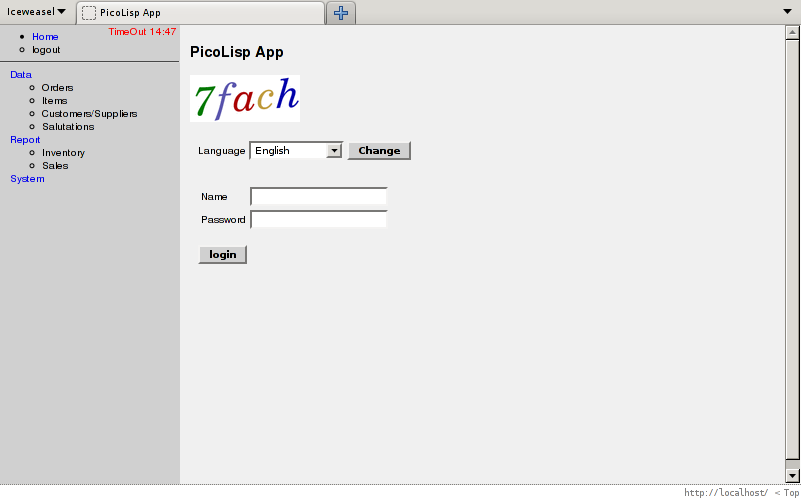
\includegraphics[scale=.4]{graphics/gui-script1.jpg}
\end{figure}


log in on the first page (by typing user name and password, and pressing the
``login'' button),

\begin{figure}[H]
\centering
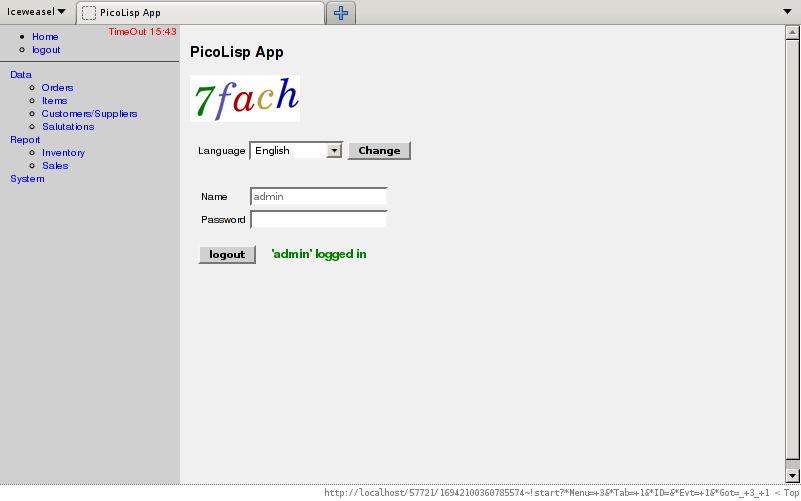
\includegraphics[scale=.4]{graphics/gui-script2.jpg}
\end{figure}


then search for that article in the ``Items'' search dialog (after clicking on the
``Items'' link in the ``Data'' submenu),

\begin{figure}[H]
\centering
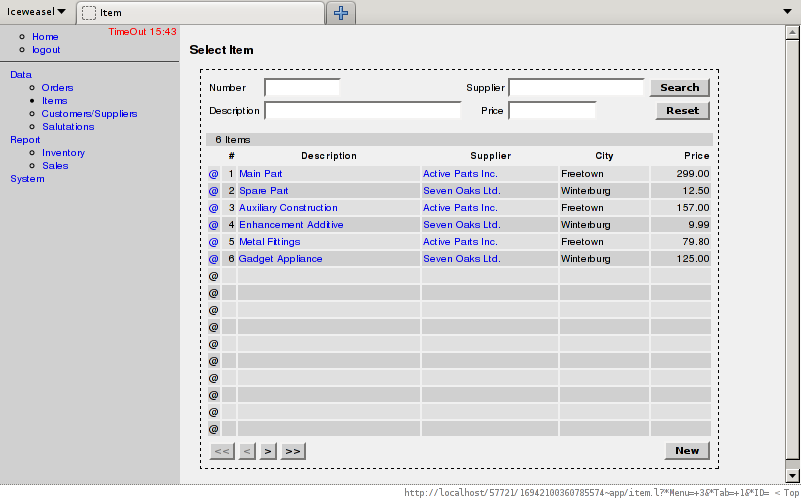
\includegraphics[scale=.4]{graphics/gui-script3.jpg}
\end{figure}


and read the price on the page of that item (here: 12.50).

\begin{figure}[H]
\centering
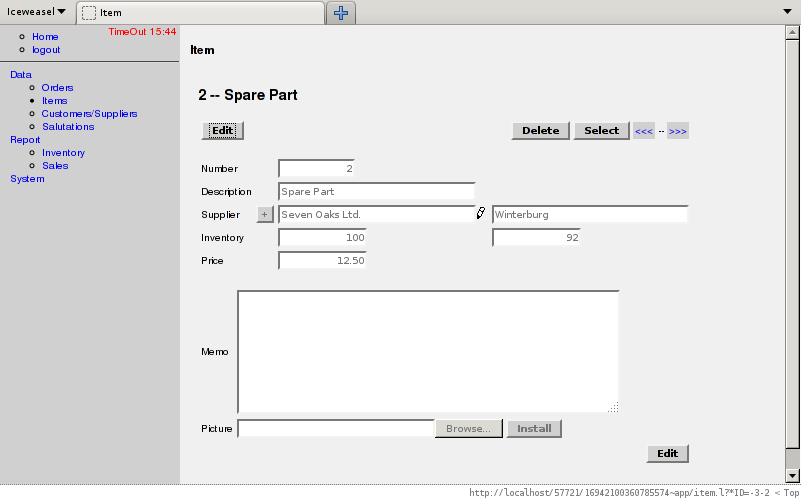
\includegraphics[scale=.4]{graphics/gui-script4.jpg}
\end{figure}


\subsection{Using GUI Scripting}
\label{sec:gui-script-using-gui-scripting}

The same result can be obtained without a browser, by interacting on
the REPL with the remote application. We assume that the demo
application is still running locally at
\underline{http://localhost:8080}\footnote{http://localhost:8080}.

Start PicoLisp, and load the necessary libraries:
\begin{wideverbatim}
   $ pil +
   : (load "@lib/http.l" "@lib/scrape.l")
\end{wideverbatim}

Call \texttt{scrape} to connect to the server
\begin{wideverbatim}
   : (scrape "localhost" 8080)
   -> "PicoLisp App"
\end{wideverbatim}

If you must use the online demo server, call \texttt{(scrape
  "7fach.de" 80 "8080")} instead, telling \texttt{scrape} to connect
to port 80 of that server (where 'httpGate' is running), and then to
dispatch to 8080 (the application's address).

Now log in:
\begin{wideverbatim}
   : (expect "'admin' logged in"
      (enter 3 "admin")
      (enter 4 "admin")
      (press "login") )
   -> NIL
\end{wideverbatim}

(\textbf{Caveat}: Keep in mind a fundamental feature of the PicoLisp
server: Whenever a second log in of the same user from the same IP
address is detected, the first session of that user is automatically
terminated. This means that you cannot run a GUI and a \texttt{scrape}
session with user ``admin'' at the same time. If you already had a gui
session open, it will be \textit{dead} now.)

\texttt{expect} takes a string argument -- a pattern which is to be
expected on the resulting page after the body (the remaining
arguments) was executed. This body enters two values (the user name
and the password) into the appropriate fields, and presses the
``login'' button.

\texttt{enter} takes a field specification and a value. The first call
with \texttt{3} refers to the ``Name'' field, as this is the third
field on the form (the first field is the ``TimeOut'' indicator, and
the second one is the language selector). The next field, field number
\texttt{4}, is the password field.

Finally, \texttt{press} simulates a press of the corresponding button,
and the message ``'admin' logged in'' appears on the page, satisfying
\texttt{expect}.

Then, just as in the GUI, click on the ``Items'' link to open the
dialog. We forgo the \texttt{expect} here, and assume that the dialog
can't fail:

\begin{wideverbatim}
   : (click "Items")
   -> "Item"
\end{wideverbatim}

We also assume that ``Spare Part'' readily appears in the result list
of the search dialog (it was on the second line). A real script would
interact with the dialog to find the desired item. So we just click on
it:

\begin{wideverbatim}
   : (click "Spare Part")
   -> "Item"
\end{wideverbatim}

Now the page of that article is open. Counting the fields, we find
that the price is in the 8th one. We can read that field's value, and
get the same result as in the GUI session above:

\begin{wideverbatim}
   : (value 8)
   -> "12.50"
\end{wideverbatim}

Note that you can also get an overview of the current page with
\texttt{display}:

\begin{wideverbatim}
: (display)
###############
click "Home" "logout" "Data" "Orders" "Items" "Customers/Suppliers"
"Salutations" "Report" "Inventory" "Sales" "System" "<<<" ">>>" "obj"

press "Edit" "Delete" "Select" "+" "Install" "Edit"

value "TimeOut 12:11" "2" "Spare Part" "Seven Oaks UnLtd." "Winterburg" "100"
"98" "12.50"

-> "Item"
\end{wideverbatim}

This helps you to find the positions of links, buttons and fields.

Finally, we should log out:
\begin{wideverbatim}
   : (click "logout")
   -> "PicoLisp App"
\end{wideverbatim}


\section{The Scrape Library}
\label{sec:gui-script-the-scrape-library}

To use the GUI scripting functionality, you need to load
``@lib/http.l`` and ``@lib/scrape.l``. It implements the following
functions:

\begin{itemize}
\item \texttt{(scrape 'host 'port 'how) -> sym | lst} Sets up an
  environment for further operations on an application, which can be
  \texttt{connect}ed on a server at \texttt{host} and \texttt{port},
  and an optional URL argument \texttt{how}. Returns the title of the
  page if no errors occurred, otherwise a list of error messages.

\item \texttt{(expect 'sym . prg)} Executes a \texttt{prg} body
  (holding calls to the functions explained below), and checks for an
  expected pattern \texttt{sym} in the server output.

\item \texttt{(click 'label ['cnt]) -> sym | lst} Simulates the click
  on a link. The first (or \texttt{cnt}'th) link found on the page
  which has \texttt{label} as a prefix is used. Returns the result of
  \texttt{scrape}.

\item \texttt{(press 'label ['cnt]) -> sym | lst} Simulates the press
  of a button. The first (or \texttt{cnt}'th) button found on the page
  which has \texttt{label} as a prefix is used. Returns the result of
  \texttt{scrape}.

\item \texttt{(value 'field ['cnt]) -> sym} Returns the current value
  of the GUI field. The \texttt{field} argument may be either a
  positive number (to specify the \texttt{cnt}'th field on the page),
  a negative number (to specify the \texttt{-cnt}'th last field on the
  page), or the field's name. If the name is given, then \texttt{cnt}
  may specify the form if more than one form is on the page.

\item \texttt{(enter 'field 'sym ['cnt]) -> sym} Enters a value
  \texttt{sym} into the GUI field. The \texttt{field} argument may be
  either a positive number (to specify the \texttt{cnt}'th field on
  the page), a negative number (to specify the \texttt{-cnt}'th last
  field on the page), or the field's name. If the name is given, then
  \texttt{cnt} may specify the form if more than one form is on the
  page.

\item \texttt{(display) -> sym} Display the state of the current page.
  First a line \texttt{\#\#\#\#\#\#\#\#\#\#\#\#\#\#\#} is printed as a visual
  separator, then all available links and buttons, and the values of
  all GUI fields is printed.

\end{itemize}

All these functions can be used interactively (e.g. during development
and debugging of a script), and in stand-alone programs. In the latter
case, they can be used as building-blocks of higher-level functions,
to interact flexibly with forms, dialogs and alerts.

Let your imagination fly!

